\documentclass[unicode,11pt,a4paper,oneside,numbers=endperiod,openany]{scrartcl}

\usepackage{ifthen}
\usepackage[utf8]{inputenc}
\usepackage{graphics}
\usepackage{graphicx}
\usepackage{hyperref}

\pagestyle{plain}
\voffset -5mm
\oddsidemargin  0mm
\evensidemargin -11mm
\marginparwidth 2cm
\marginparsep 0pt
\topmargin 0mm
\headheight 0pt
\headsep 0pt
\topskip 0pt        
\textheight 255mm
\textwidth 165mm

\newcommand{\duedate} {}
\newcommand{\setduedate}[1]{%
\renewcommand\duedate {Due date:~ #1}}
\newcommand\isassignment {false}
\newcommand{\setassignment}{\renewcommand\isassignment {true}}
\newcommand{\ifassignment}[1]{\ifthenelse{\boolean{\isassignment}}{#1}{}}
\newcommand{\ifnotassignment}[1]{\ifthenelse{\boolean{\isassignment}}{}{#1}}

\newcommand{\assignmentpolicy}{
\begin{table}[h]
\begin{center}
\scalebox{0.8} {%
\begin{tabular}{|p{0.02cm}p{16cm}|}
\hline
&\\
\multicolumn{2}{|c|}{\Large\textbf{HPC Lab 2020 ---  Submission Instructions}}\\
\multicolumn{2}{|c|}{\large\textbf{(Please, notice that following instructions are mandatory: }}\\
\multicolumn{2}{|c|}{\large\textbf{submissions that don't comply with, won't be considered)}}\\
&\\
\textbullet & Assignments must be submitted to \href{https://www.icorsi.ch/course/view.php?id=10049}{Icorsi} (i.e. in electronic format).\\
\textbullet & Provide both executable package and sources (e.g. C/C++ files, Matlab). 
If you are using libraries, please add them in the file. Sources must be organized in directories called:\\
\multicolumn{2}{|c|}{\textit{Project\_number\_lastname\_firstname}}\\
& and  the  file must be called:\\
\multicolumn{2}{|c|}{\textit{project\_number\_lastname\_firstname.zip}}\\
\multicolumn{2}{|c|}{\textit{project\_number\_lastname\_firstname.pdf}}\\
\textbullet &  The TAs will grade your project by reviewing your project write-up, and looking at the implementation 
                 you attempted, and benchmarking your code's performance.\\

\textbullet & You are allowed to discuss all questions with anyone you like; however: (i) your submission must list anyone you discussed problems with and (ii) you must write up your submission independently.\\
\hline
\end{tabular}
}
\end{center}
\end{table}
}
\newcommand{\punkte}[1]{\hspace{1ex}\emph{\mdseries\hfill(#1~\ifcase#1{Points}\or{Points}\else{Points}\fi)}}


\newcommand\serieheader[6]{
\thispagestyle{empty}%
\begin{flushleft}

\includegraphics[width=0.4\textwidth]{images/usi_inf.pdf}
\end{flushleft}
  \noindent%
  {\large\ignorespaces{\textbf{#1}}\hspace{\fill}\ignorespaces{ \textbf{#2}}}\\ \\%
  {\large\ignorespaces #3 \hspace{\fill}\ignorespaces #4}\\
  \noindent%
  \bigskip
  \hrule\par\bigskip\noindent%
  \bigskip {\ignorespaces {\Large{\textbf{#5}}}
  \hspace{\fill}\ignorespaces \large \ifthenelse{\boolean{\isassignment}}{\duedate}{#6}}
  \hrule\par\bigskip\noindent%  \linebreak
 }

\makeatletter
\def\enumerateMod{\ifnum \@enumdepth >3 \@toodeep\else
      \advance\@enumdepth \@ne
      \edef\@enumctr{enum\romannumeral\the\@enumdepth}\list
      {\csname label\@enumctr\endcsname}{\usecounter
        {\@enumctr}%%%? the following differs from "enumerate"
	\topsep0pt%
	\partopsep0pt%
	\itemsep0pt%
	\def\makelabel##1{\hss\llap{##1}}}\fi}
\let\endenumerateMod =\endlist
\makeatother




\usepackage{textcomp}





\begin{document}


\setassignment
\setduedate{20.10.2020 (midnight)}

\serieheader{High-Performance Computing Lab}{2020}{Student: Gabriele Berra}{Discussed with: -}{Solution for Project 2}{}
\newline

\assignmentpolicy
This project will introduce you to parallel programming using OpenMP.



\section{Parallel reduction operations using OpenMP [10 points]}
\subsection{Parallel version with reduction clause and with parallel and critical clauses}

The objective of this exercise was to parallelize the given dot product code by using the reduction clause and the parallel and critical clauses. As far as concerns the parallelization with the reduction clause, it has been done as follows: an additional variable named \emph{parallel\_alpha} has been introduced, so that every thread can compute its own part of the for loop and then all the intermediate results are summed up in the global variable.

Before starting the explanation of the parallelization with the clauses parallel and critical, I think is better to understand what \textit{critical} is and what is its behaviour inside a parallel region. The critical clause permits at only one thread at a time to enter a specific part of the parallel code: when the thread inside the critical has finished to do its own computation, another thread can go in and so on. The major problem using this clause is that it can compromise the performance of the parallelization if it is not called in the right place and/or with the right change in the code. Thus, to avoid that the critical clause causes any problem, I created a private variable in which I store the result of the product between $a[i] * b[i]$ in the inner for loop. After that - outside of the inner loop - I put the critical section in which every thread sums its own copy of the private variable in the global variable \textit{alpha\_parallel}. My implementation is included here below. \\

\lstinputlisting[frame=single, breaklines=true, tabsize=3, language=C++]{project2_code/dotProduct.cpp}

\vskip 0.2in

After explaining the modifications I have done to the code, we are interested in visualizing the results obtained against different numbers of threads, in order to analyze the scalability of the code. I was unsure of what graphical representation would be the best to visualize my results but, at the end, I decided to use the Matlab function \emph{surf()}, which allows us to represent the data obtained in a three dimensional space (with axes given by number of threads, size of the vector and the metric considered). In figures \ref{fig:reductionScaling} and \ref{fig:criticalScaling} we can find the scaling of the code with reduction and with critical against different number of threads and against different sizes (number of elements $N$) of the vector for which we are computing the dot product.


\begin{figure}[h!]
\centering
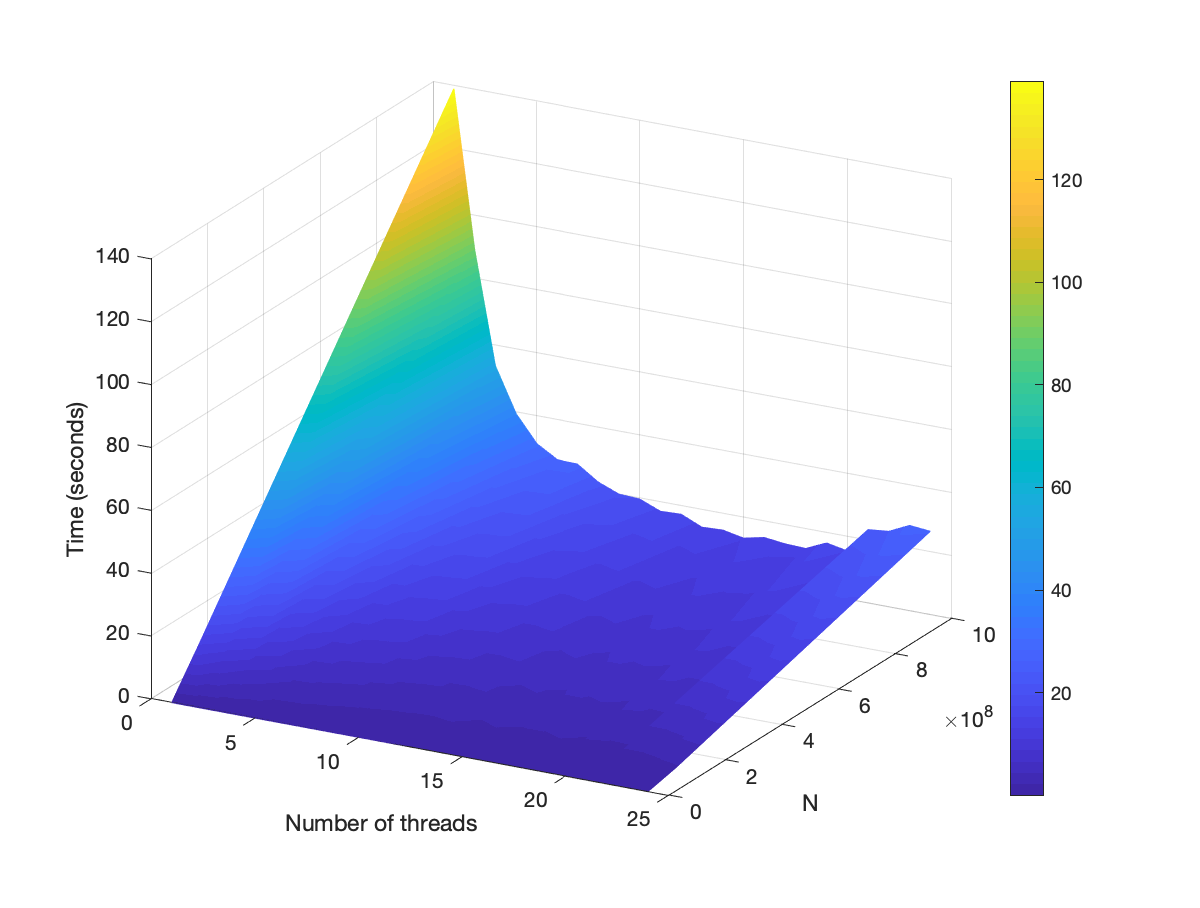
\includegraphics[width=0.6\textwidth]{Figures/surfPlot_reduction.eps}
\caption{Scaling results by using reduction against different number of threads and number of elements $N$ of the input vector.}\label{fig:reductionScaling}
\end{figure}

\begin{figure}[h!]
\centering
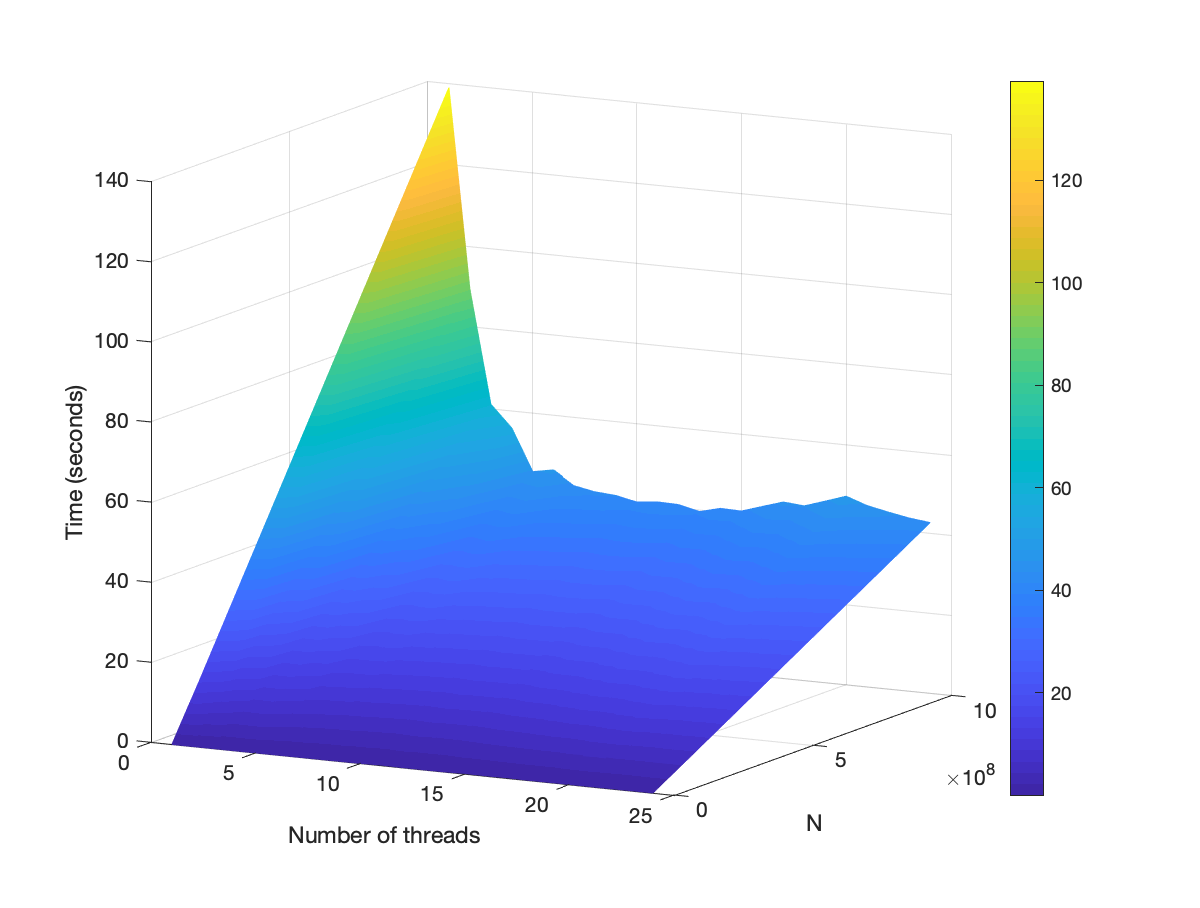
\includegraphics[width=0.6\textwidth]{Figures/surfPlot_critical.eps}
\caption{Scaling results by using critical against different number of threads and number of elements $N$ of the input vector.}\label{fig:criticalScaling}
\end{figure}

In figures \ref{fig:reductionEff} and \ref{fig:criticalEff} we can find the parallel efficiency of the code with reduction and with critical against different number of threads and against different sizes (number of elements $N$) of the vector for which we are computing the dot product. The parallel efficiency has been computed simply as the ratio between the time obtained with a single thread and the time obtained for a higher number of threads (keeping $N$ fixed).

\begin{figure}[h!]
\centering
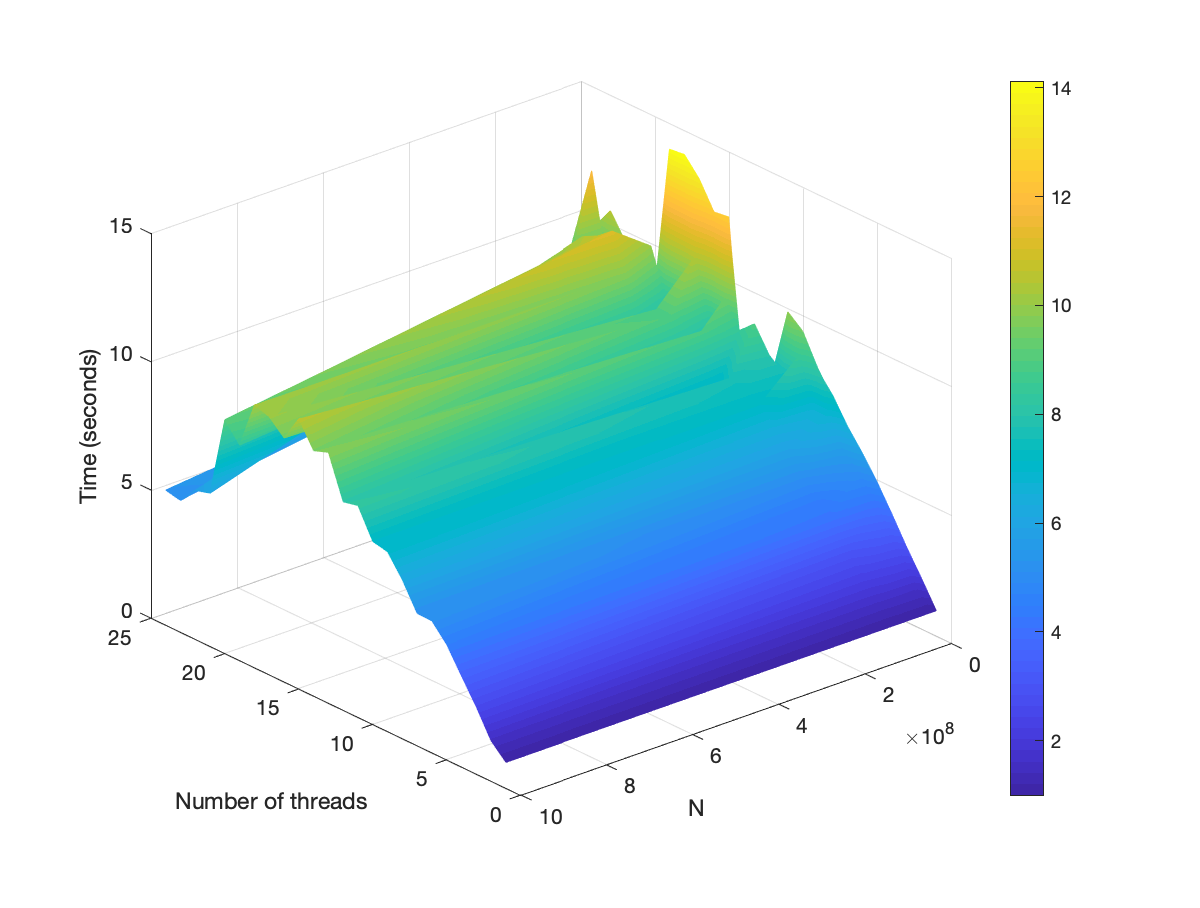
\includegraphics[width=0.6\textwidth]{Figures/surfPlot_rEff.eps}
\caption{Parallelel efficiency of the implementation using reduction against different number of threads and number of elements $N$ of the input vector.}\label{fig:reductionEff}
\end{figure}

\begin{figure}[h!]
\centering
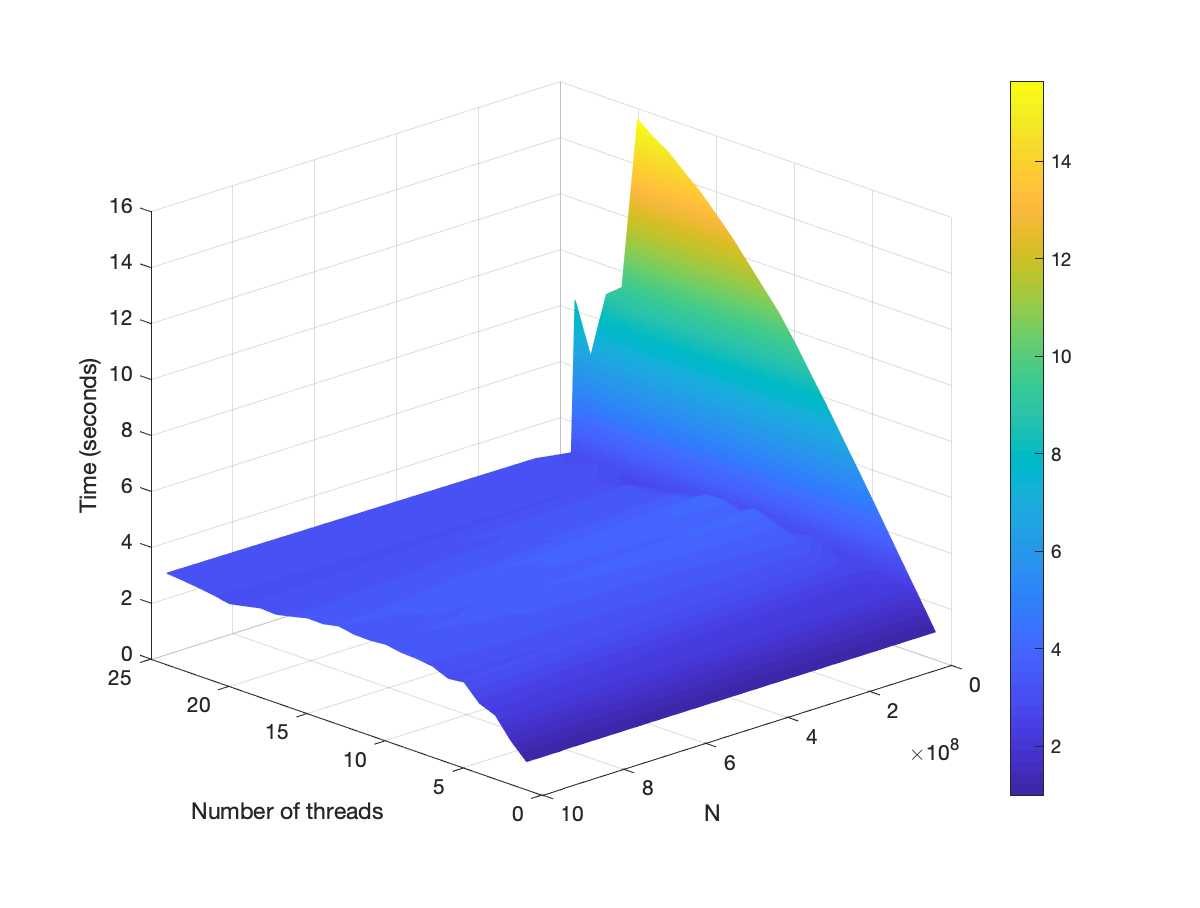
\includegraphics[width=0.6\textwidth]{Figures/surfPlot_cEff.eps}
\caption{Parallelel efficiency of the implementation using critical against different number of threads and number of elements $N$ of the input vector.}\label{fig:criticalEff}
\end{figure}

According to the results I obtained, depicted in the figures above, it would be beneficial to use a multi-threaded version of the dot product for all the cases analysed, but - in particular - starting from a size $N=10^7$, as can be noticed by observing the results with the times of the serial implementation.

\begin{figure}[h!]
\centering
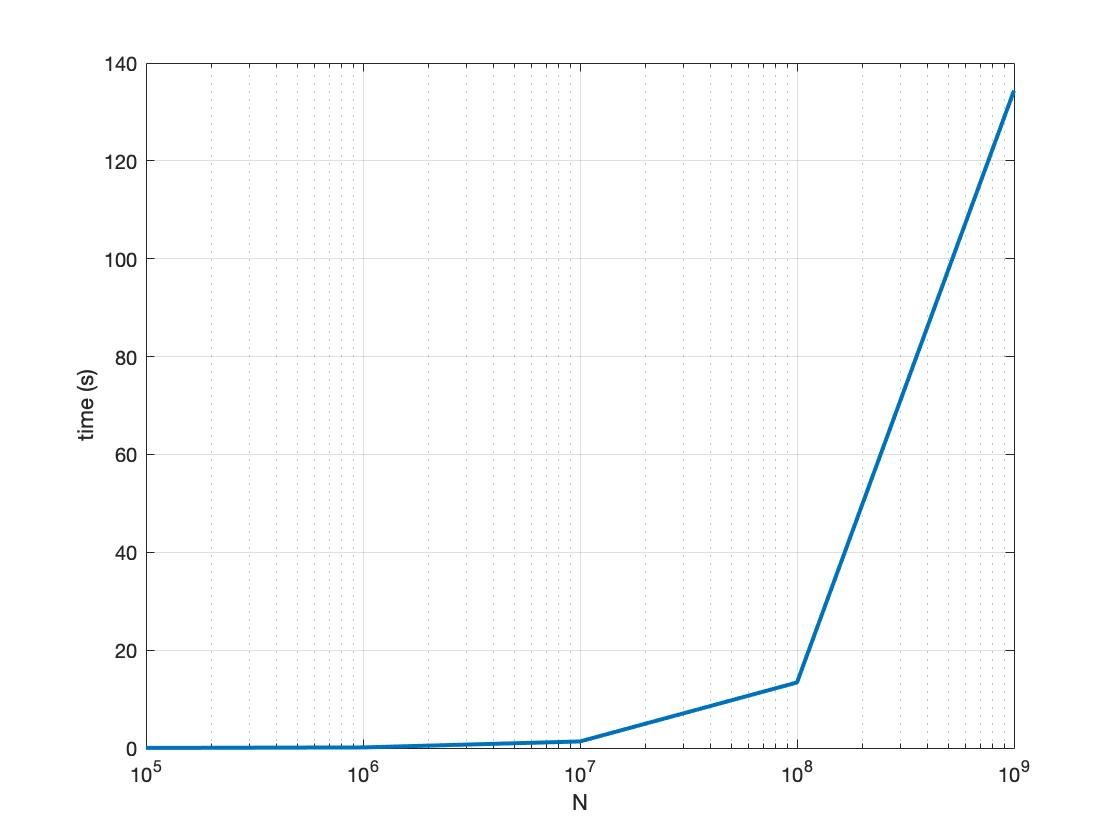
\includegraphics[width=0.6\textwidth]{Figures/serialLog.jpg}
\caption{Time required by the serial implementation against different number of elements $N$ of the input vector.}\label{fig:criticalEff}
\end{figure}

%----------------------------------------------------------------------------------------
 
\section{The Mandelbrot set using OpenMP [30 points]}
\subsection{Mandelbrot set}
In this second exercise regarding the Mandelbrot set I firstly understood the theory behind the so called "most complex object in mathematics" (James Gleick, "Chaos: Making a New Science") and, secondly, how to plot it using C. We know that the Mandelbrot set is defined as a set of complex numbers for which the sequence $z,f_c(z),f_c^2(z),f_c^3(z)...$ does not approach infinity (i.e., it remains bounded). In order to produce the plot we have to understand how the given \textit{manedl\_seq.c} code works and what are the interactions between the given variables. Mathematically we have:
\begin{equation*}
	\lim_{n \rightarrow \infty}\|z_{n+1} = z_n^2 + c \| \;\text{does not approach}\; \infty
\end{equation*}
in which the norm considered is Euclidean and simply defined as:
\begin{equation*}
	\|z\| = \sqrt{x^2 + y^2}
\end{equation*}
In the equation above, $x$ indicates the real part, while $y$ is the imaginary part. We can rewrite this equation as follows:
\begin{equation*}
	\|z\|^2 = x^2 + y^2.
\end{equation*}

After this brief recap of the theory we can proceed with the real C implementation. We know from the last equation and the theory that a given complex number belongs to the Mandelbrot set if $2 > \sqrt{x^2 + y^2}$ or $4 > x^2 + y^2$. In my code, I implemented a \textit{while loop} which takes into consideration the maximum number of iterations and the boundary of the Mandelbrot set. In the loop I incremented the value of $x$ and $y$ so that, at every iteration, they are updated and ready to check if in the two constraint are satisfied and if the number belongs to the set. \\

% TODO: Add code here
\lstinputlisting[frame=single, breaklines=true, tabsize=3, language=C]{project2_code/mandel_seq.c}


\subsection{Mandelbrot set: parallelization}
With the aim of parallelizing the Mandelbrot set I used the \textit{reduction clause} in a \textit{parallel for} section. This approach produced the correct result in almost every pixel, despite a few one which were suppose to be black instead of white and vice versa. This error is called a \textit{race condition} and the understanding of this problem is crucial to arrive at the correct result. Basically when we write a simple code without parallelization we use only one thread which performs all the calculations. In contrast, in a "parallel code", the \textit{master thread} - i.e. the thread that performs the calculations in the non-parallelized section - whenever it hits a parallel section, splits itself and creates a \textit{thread team} that works together to perform the computations. In the parallel section, sometimes, two threads work with the same variable and it could happen that the second overwrites the value of the first one: this situation is the so-called \textit{race condition}. In order to avoid it, I had to set all the variable as private: in this way, every thread has its own copy of the variable and, thus, the race condition is no longer possible. \\


\lstinputlisting[frame=single, breaklines=true, tabsize=3, language=C]{project2_code/mandel_par.c}

To conclude this section, I want to present the results obtained by running the serial version of the Mandelbrot set against the parallelized version which I implemented. As we can see from figure \ref{fig:mandelbrot}, the time (in milliseconds) required by the serial version quickly increases when the size of the picture increases. On the contrary, the parallelized version performs way better and allows us to obtain the same output (i.e., the graphical representation o the Mandelbrot set) in a significantly lower time.

\begin{figure}[h]
\centering
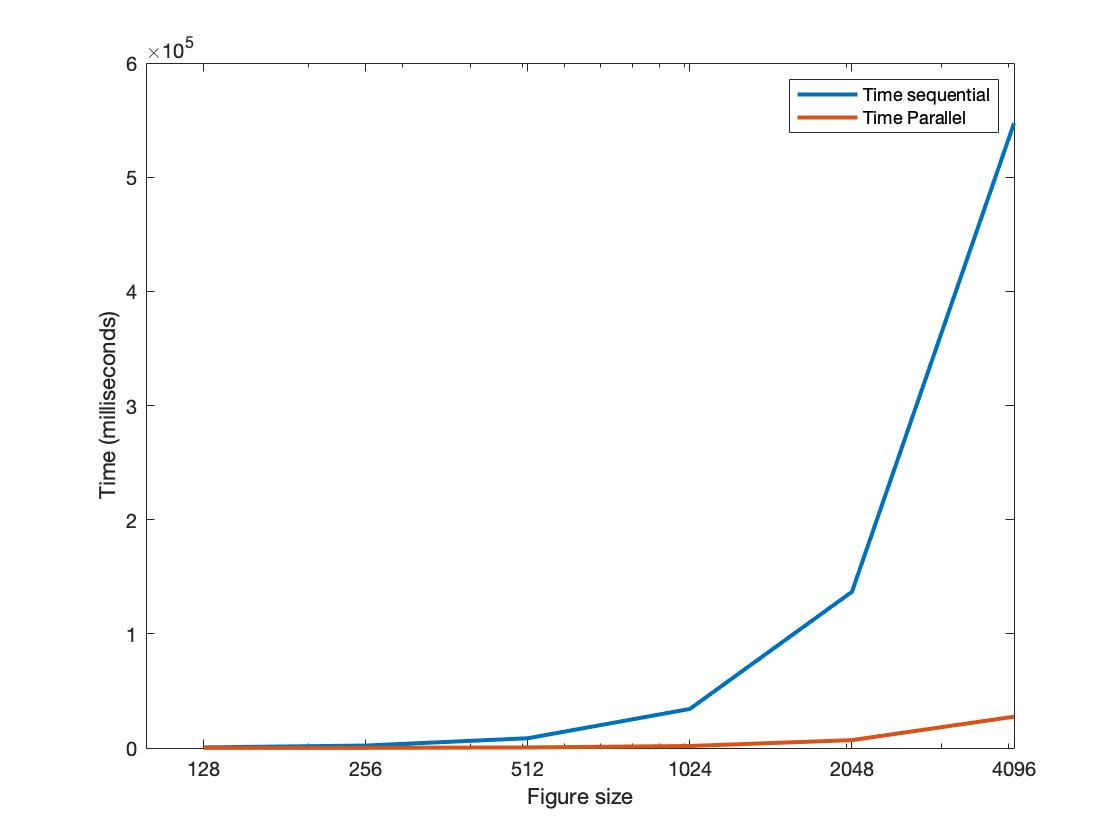
\includegraphics[width=0.75\textwidth]{Figures/timing_mandelbrot.jpg}
\caption{Serial versus parallelized Mandelbrot against different image sizes.}\label{fig:mandelbrot}
\end{figure}


%--------------------------------------------------------------------------------------

\section{Bug hunt [20 points]}
\subsection{omp\_bug1.c}
In the first script, the error is that the \textit{pragma omp parallel for} has to be declared just before the for loop. In this case, in order to solve the problem, I suggest to move the omp declaration just before the for loop and also to remove the curly brackets because they give an error in function main, line 27. With the removal of the curly brackets, the code works as expected.\\

\lstinputlisting[frame=single, breaklines=true, tabsize=3, language=C]{project2_code/omp_bug1.c}

\subsection{omp\_bug2.c}
The second script should print, for every thread, both when it begins to do its job and when it has finished to do its computations. The bug is that only the last thread is printed at the end of the computation. The solution is to privatize the variable \textit{tid} and \textit{total}, so that every thread has its own copy of the variable.\\

\lstinputlisting[frame=single, breaklines=true, tabsize=3, language=C]{project2_code/omp_bug2.c}

\subsection{omp\_bug3.c}  
In this third code, we can easily notice that the program never terminates its execution. We know from the theory that the barrier clause is used to "stop" the threads and wait until all of them have finished their work: afterwards, once they have been all synchronised, they can continue with the computations in the parallel section. In this specific code, the problem is relative to the number of barriers that the threads hit before the end of the program. At the end of the program, N-2 threads hit a barrier less than the others and, thus, we reach a situation of stall in which they keep waiting for the other two threads, that will however never come. In order to solve this bug we just have to remove the \textit{\#pragma omp barrier} in the \textit{print\_results()}. By removing this last barrier, every thread hits - during the computations - the same number of barriers, thus solving the bug.\\

\lstinputlisting[frame=single, breaklines=true, tabsize=3, language=C]{project2_code/omp_bug3.c}

\subsection{omp\_bug4.c}
If we run this fourth code, we encounter a \textit{Segmentation fault (core dumped)}. After doing some research, I found that the maximum stack of one ICS cluster node is 8192 kbytes, which means that, in the code, I cannot allocate more than the 8192 kbytes of data. The variable $a$ is an $NxN$ matrix of doubles (8 bytes each) and N is 1048., thus leading to:
\begin{equation*}
	1048 * 1048 * 8 = 9786432\;\; \text{bytes or}\;\; 8580.5 \;\;\text{kbytes} 
\end{equation*}
which exceeds the maximum of the ICS cluster.
In order to solve this bug we have to set $N$ to the maximum value allowed for the given stack size, i.e. we have to set $N=1023$.\\

\textit{Remark}: If we try to run the code with $N = 1024$ the result is a segmentation fault of the same type of the previous one. This is because the weight of the matrix in terms of kbytes is exactly 8192, but since we have to save not only the matrix (but also, e.g., the indices of the matrix), 8192 kbytes are not enough.\\

\lstinputlisting[frame=single, breaklines=true, tabsize=3, language=C]{project2_code/omp_bug4.c}

\subsection{omp\_bug5.c}
Finally the last bugged code is a neverending program. This problem is caused by an overlap of two open locks which cannot permit to the threads to continue with their computation. This problem can be easily solved by separating the locks and not nesting one inside the other as follows:\\

\lstinputlisting[frame=single, breaklines=true, tabsize=3, language=C]{project2_code/omp_bug5.c}





\section{Parallel histogram calculation using OpenMP [20 points]}
In the parallelization of the histogram calculation I used a reduction clause that allowed me to reduce the time for the computations. In table \ref{tab:hist} we can find the results of the parallelization with up to 10 threads (please notice that the serial execution of the original implementation is MANCA). In figure \ref{fig:histScaling} we can observe a graphical representation of the scaling results for up to 10 threads: in particular, we can observe that we gain a significant reduction of the computational till up to 5 threads, while afterwards the gains start to decrease. The latter behaviour could be explained as a consequence of the relative small size of our input: in other words, initializing too many threads offsets somehow the advantages of parallelizing our application, given the size of the problem.

\lstinputlisting[frame=single, breaklines=true, tabsize=3, language=C++]{project2_code/hist_omp.cpp}

\begin{table}
\begin{center}
	\begin{tabular}{|c|c|}
		\hline
		%\multicolumn{2}{|c|}{Hist parallelization} \\
		\textbf{\# Threads} & \textbf{Time(s)}\\
		\hline\hline
		1 & 0.826919  \\
		\hline
		2  & 0.438337  \\
		\hline
		3  & 0.291285  \\
		\hline
		4  & 0.219064  \\
		\hline
		5  & 0.17477  \\
		\hline
		6  & 0.144787  \\
		\hline
		7  & 0.124644  \\
		\hline
		8  & 0.10845  \\
		\hline
		9  & 0.0976775  \\
		\hline
		10  & 0.0879112  \\
		\hline
	\end{tabular}
\end{center}
\caption{Time required for the histogram computation with different numbers of threads.}\label{tab:hist}
\end{table}


\begin{figure}[h]
\centering
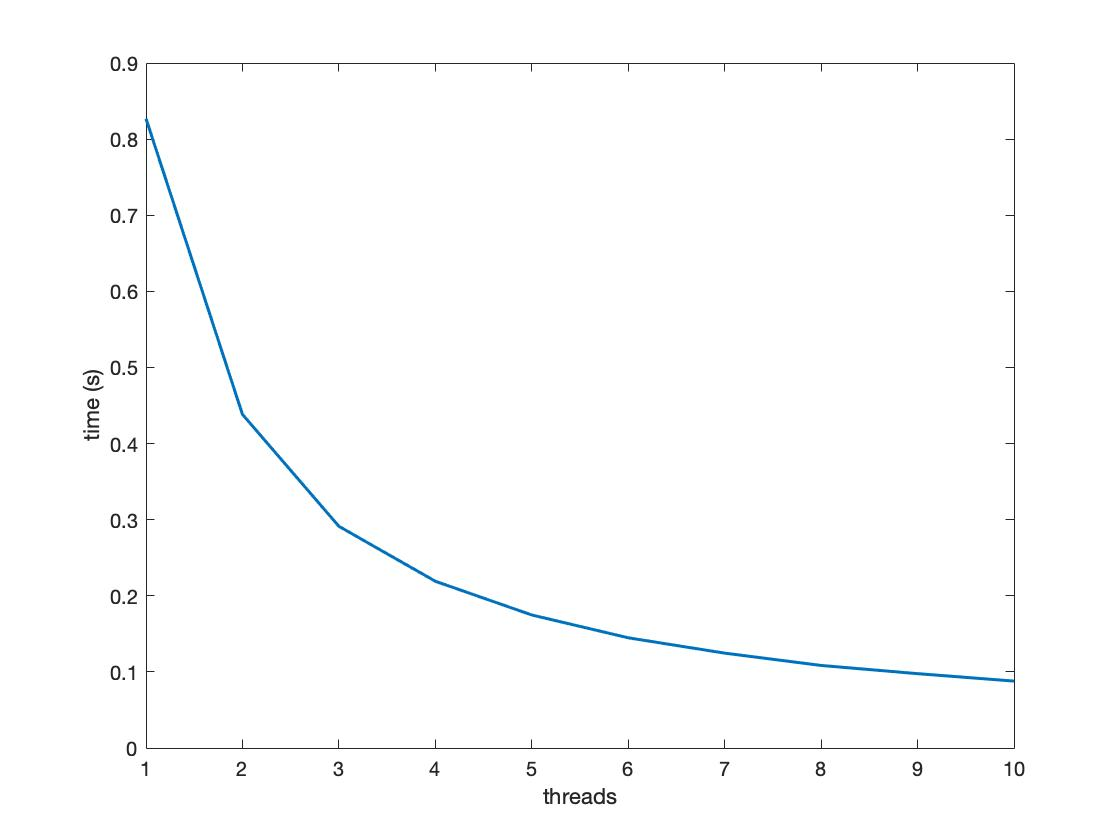
\includegraphics[width=0.75\textwidth]{Figures/histTimes.jpg}
\caption{Scaling results for the histogram computation with different number of threads.}\label{fig:histScaling}
\end{figure}





\section{Parallel loop dependencies with OpenMP [20 points]}
We know from the theory that, in some cases, it is not trivial to parallelize a for loop, especially in the case of a loop-dependant variable. In other words, a possible scenario is that in the $n+1$ iteration we need a variable that has been computed in the previous iteration $n$. In these cases, the first thing that we have to do is solving the dependence between the variables. and then start the parallelization. In our case the code creates a pointer vector (opt) in which:

\begin{equation*}
	opt[n+1] = opt[n] * up
\end{equation*}
In order to solve this problem, my first attempt consisted in simply using the \textit{pow()} function, in order to compute - at every iteration -  the exact value at position $n$ of the pointer vector. By doing so, I - however - realized that the repeated calls to the function \textit{pow()} were significantly expensive and my code was actually performing worse than the serial version, despite the parallelization.

In the second version of my code, I decided then to minimize the utilisation of the \textit{pow()} function by adding an \textit{if ... else} construct in which only the first computation of each thread would use the function and, after that, the computations would be carried over with the regular $Sn * up$ defined above. The results obtained for a number of threads ranging from 1 to 18 are summarized in table \ref{tab:recursive}. In figure \ref{fig:recurScaling} we can find a graphical representation of the results obtained: as happened in the previous exercise, we can notice a significant scaling of our parallelized code up to 5 threads, after which number the performance starts to decrease (and what is gained from adding an additional thread is only a small speed up).

\vskip 0.25in
\lstinputlisting[frame=single, breaklines=true, tabsize=3, language=C]{project2_code/recur_omp.c}

\begin{table}[h]
\begin{center}
	\begin{tabular}{|c|c|}
		\hline
		\textbf{\# Threads} & \textbf{Time(s)}\\
		\hline\hline
		1  & 6.715699  \\
		\hline
		2  & 3.377089  \\
		\hline
		4  & 1.690796  \\
		\hline
		6  & 1.132449  \\
		\hline
		8  & 0.857513  \\
		\hline
		10  & 0.724234  \\
		\hline
		12  & 0.597950  \\
		\hline
		14  & 0.569803  \\
		\hline
		16  & 0.521026  \\
		\hline
		18  & 0.517610  \\
		\hline
	\end{tabular}
\caption{Time required for the recursion code with different numbers of threads.}\label{tab:recursive}
\end{center}
\end{table}

\begin{figure}[h]
\centering
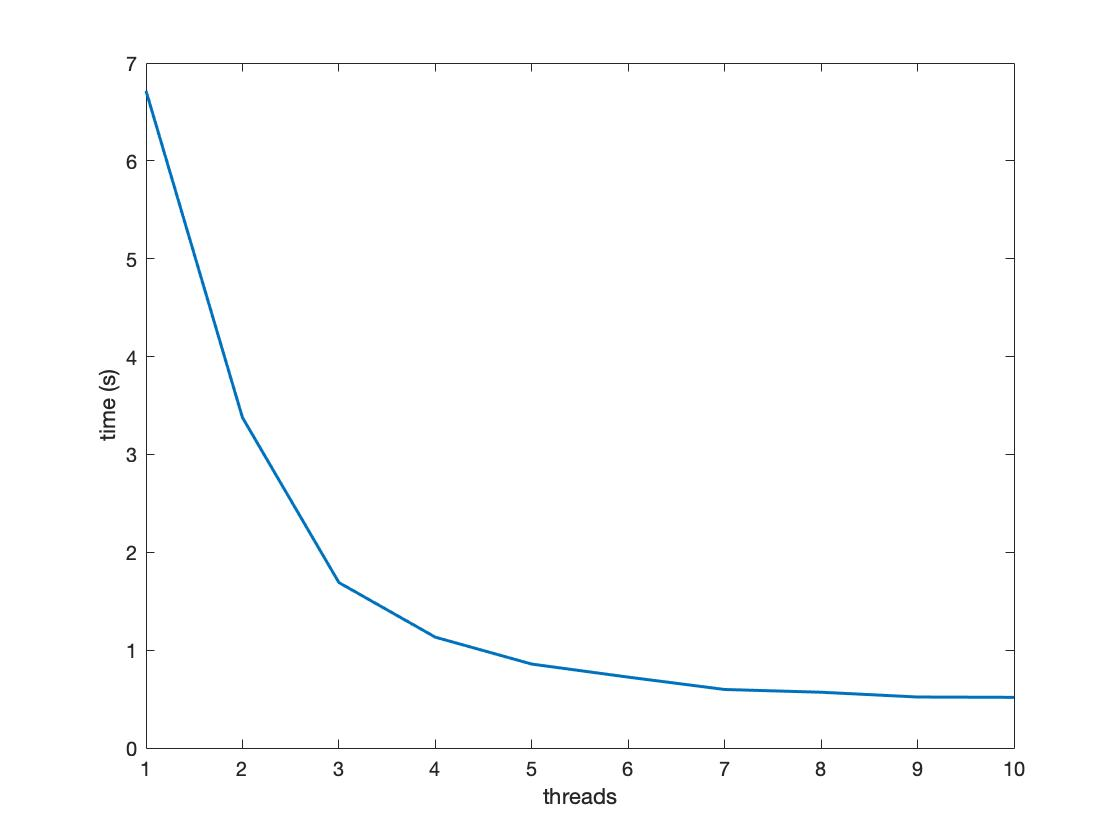
\includegraphics[width=0.75\textwidth]{Figures/recurScaling.jpg}
\caption{Scaling results for the recursion code with different number of threads.}\label{fig:recurScaling}
\end{figure}























\end{document}
